\documentclass[conference]{IEEEtran}
\IEEEoverridecommandlockouts
% The preceding line is only needed to identify funding in the first footnote. If that is unneeded, please comment it out.
% \usepackage{cite}
\usepackage{amsmath,amssymb,amsfonts}
\let\OldAngle\angle
\renewcommand{\angle}{\anglesym}

\usepackage{rotating}
\usepackage{graphicx}
\usepackage{balance}

\usepackage{epstopdf}
\epstopdfsetup{outdir=./}

\usepackage{natbib}
\bibpunct{[}{]}{;}{n}{,}{,} % required for natbib

\usepackage{multirow,tabularx}
% \usepackage{SIunits}
\usepackage{xspace}
\usepackage[table]{xcolor}% http://ctan.org/pkg/xcolor

\usepackage{hyperref}
\usepackage{hypcap} % Correct a problem with hyperref

\usepackage{circuitikz}
\usetikzlibrary{arrows}
\usepackage[justification=raggedright,font=small]{caption}
\usepackage{subcaption}

\usepackage[free-standing-units]{siunitx}
\usepackage{cleveref}% load last

\usepackage{mathtools}

\crefname{equation}{equation}{eq. }
\Crefname{equation}{Eq.}{Eq.}% For beginning \Cref
\crefrangelabelformat{equation}{(#3#1#4--#5#2#6)}

\crefmultiformat{equation}{eq. #2#1#3}{, #2#1#3}{#2#1#3}{#2#1#3}
\Crefmultiformat{equation}{Eq. #2#1#3}{, #2#1#3}{#2#1#3}{#2#1#3}

%\usepackage{pdfcomment}

% PDFCOMMENT EXAMPLES:

% You can do much more \pdfmarkupcomment[markup=Squiggly,color=green,author=CAP]{with pdfcomment}{move to the front}.
% This is a \pdfmarkupcomment[markup=StrikeOut,color=red,author=CAP]{stupid}{replace stupid with funny}  game!
% \pdfmarkupcomment[markup=Highlight,color=yellow,author=CAP]{Of course, you can highlight complete sentences.}{Highlight}
% This is very\pdfcomment[icon=Note,color=blue]{insert graphic!} interesting!

\newcommand{\specialcell}[2][c]{%
  \begin{tabular}[#1]{@{}l@{}}#2\end{tabular}}

\newcommand\redbox[3][red]{\textcolor{#1}{\rule{#2}{#3}}}

\newcommand{\brieftbllink}[1]{\hyperref[#1]{Tbl.~\ref*{#1}}\xspace }
\newcommand{\briefeqlink}[1]{\hyperref[#1]{Eq.~\ref*{#1}}\xspace }
\newcommand{\tablelink}[1]{\hyperref[#1]{Tbl.~\ref*{#1}}\xspace }
\newcommand{\eqlink}[1]{\hyperref[#1]{Equation~\ref*{#1}}\xspace }
\newcommand{\briefseclink}[1]{\hyperref[#1]{Sec.~\ref*{#1}}}
\newcommand{\seclink}[1]{\hyperref[#1]{Section~\ref*{#1}}}
\newcommand{\parbreak}{\ \\
\noindent}
\newcommand{\brieffiglink}[1]{\hyperref[#1]{Fig.~\ref*{#1}}}
\newcommand{\brieffigsublink}[2]{\hyperref[#1]{Fig.~\ref*{#1}#2}}

\newcommand{\vulgaronehalf}{${}^1\!\!\mskip0.3\thinmuskip/\!{}_2$}


\title{Practical Measurement of Voltage-Controlled Current Source Output Impedance for Applications in Transcranial Electrical Stimulation}

\author{\IEEEauthorblockN{Charl Linssen}
\IEEEauthorblockA{\textit{Donders Institute for Brain, Cognition and Behaviour} \\
\textit{Radboud University Nijmegen} \\
Nijmegen, The Netherlands\\
c.linssen@donders.ru.nl}
\and
\IEEEauthorblockN{Pieter Harpe}
\IEEEauthorblockA{\textit{Integrated Circuits Group} \\
\textit{Eindhoven University of Technology}\\
Eindhoven, The Netherlands \\
p.j.a.harpe@tue.nl}\\
\ \\
2021 IEEE Biomedical Circuits and Systems Conference (BioCAS)\\
October 6--9, 2021
}

%%%%%%%%%%%%%%%%%%%%%%%%%%%%%%%%%%%%%%%%%%%%%%%%%%%%%%%%%%%%%%%%%%%%%%%%%%%%%%
%%%%%%%%%%%%%%%%%%%%%%%%%%%%%%%%%%%%%%%%%%%%%%%%%%%%%%%%%%%%%%%%%%%%%%%%%%%%%%
\begin{document}

\maketitle

%%%%%%%%%%%%%%%%%%%%%%%%%%%%%%%%%%%%%%%%%%%%%%%%%%%%%%%%%%%%%%%%%%%%%%%%%%%%%%
%%%%%%%%%%%%%%%%%%%%%%%%%%%%%%%%%%%%%%%%%%%%%%%%%%%%%%%%%%%%%%%%%%%%%%%%%%%%%%
\begin{abstract}
\noindent A voltage-controlled current source (VCCS) is a key component in the electrical stimulation of neuronal tissue. We present a method for the evaluation of output impedance across frequency, of VCCS circuits with applications in transcranial electrical stimulation (tES). Two VCCS circuit architectures, one with a single-ended, and one with a differential output, are theoretically analysed and simulated, and the method is validated by matching these results with empirical measurements. Monte Carlo simulation of the measurement method itself is used to predict its range of applicability under real-world conditions. Both circuits, as well as the method used to determine output impedance, are easy to reproduce, using generic hardware components at low cost. The method described has immediate practical application value in neuroscience research, where it can be used in the deployment and further development of VCCS circuit architectures.
\end{abstract}


%%%%%%%%%%%%%%%%%%%%%%%%%%%%%%%%%%%%%%%%%%%%%%%%%%%%%%%%%%%%%%%%%%%%%%%%%%%%%%
%%%%%%%%%%%%%%%%%%%%%%%%%%%%%%%%%%%%%%%%%%%%%%%%%%%%%%%%%%%%%%%%%%%%%%%%%%%%%%
\begin{IEEEkeywords}
neuromodulation, neural, transcranial, current source
\end{IEEEkeywords}


%%%%%%%%%%%%%%%%%%%%%%%%%%%%%%%%%%%%%%%%%%%%%%%%%%%%%%%%%%%%%%%%%%%%%%%%%%%%%%
\section{Motivation}
\label{sec:motivation}
%%%%%%%%%%%%%%%%%%%%%%%%%%%%%%%%%%%%%%%%%%%%%%%%%%%%%%%%%%%%%%%%%%%%%%%%%%%%%%

Transcranial electrical stimulation (tES) is a relatively non-invasive way of altering the excitability of the brain. A direct, alternating or noise current (tDCS, tACS or tRNS, respectively) is delivered between two electrodes that have been placed into conductive contact with the subject's skin, on or near the scalp (\brieffiglink{fig:situation_sketch}, top). Bandwidth of the stimulation is typically below $1~\kilo\hertz$ and currents are below $2~\milli\ampere$ \cite{pmid26652115}\cite{pmid19109497}.

\begin{figure}[bt]
	\begin{subfigure}{\textwidth}
        
\hspace{-4.8cm}\makebox[\textwidth][c]{%
		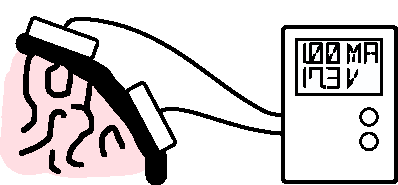
\includegraphics[scale=1.1]{fig_situation_sketch.pdf}
        }
        \caption*{}
        \label{fig:situation_sketch1}
    \end{subfigure}

	\begin{subfigure}{\textwidth}

\hspace{-4.5cm}\makebox[\textwidth][c]{%
\begin{circuitikz}
	\node [] (topleft) at (-1, 1) {};
	\node [] (bottomleft) at (-1, -1) {};

	\node [] (topright) at (2, 1) {};
	\node [] (bottomright) at (2, -1) {};

	\node [] (topright1) at (4, 1) {};
	\node [] (bottomright1) at (4, -1) {};

	\node [] (topright2) at (5, 1) {};
	\node [] (bottomright2) at (5, -1) {};

	\draw (topleft.center) to [generic, l=$Z_L$]  (bottomleft.center) {};
	\draw (bottomright1.center) to [generic, l=$Z_{out}$, *-*]  (topright1.center) {};
	\draw (bottomright2.center) to [american controlled current source, l_=$g_m$]  (topright2.center) {};
	\draw (topleft.center) to [generic, l=$Z_{elec}$, i<^=$I_L$]  (topright.center) {};
	\draw (bottomleft.center) to [generic, l=$Z_{elec}$]  (bottomright.center) {};
	\draw (topright.center) to [short] (topright1.center) {};
	\draw (bottomright.center) to [short] (bottomright1.center) {};
	\draw (topright1.center) to [short] (topright2.center) {};
	\draw (bottomright1.center) to [short] (bottomright2.center) {};

	%
	% 	RC poles: box
	%

	\node [] (vboxtr) at (2.75, 1.4) {};
	\node [] (vboxbr) at (2.75, -1.4) {};
	\node [] (vboxtl) at (6.25, 1.4) {};
	\node [] (vboxbl) at (6.25, -1.4) {};

	\draw[dashed] (vboxtr.center) to [short] (vboxbr.center) {};
	\draw[dashed] (vboxbr.center) to [short] (vboxbl.center) {};
	\draw[dashed] (vboxbl.center) to [short] (vboxtl.center) {};
	\draw[dashed] (vboxtl.center) to [short] (vboxtr.center) {};
\end{circuitikz}

}
        \caption*{\small}
        \label{fig:situation_sketch2}
    \end{subfigure}
\caption{\small Situation sketch (top panel) and equivalent circuit (bottom panel). In a typical tES session, the device is adjusted to supply a given current $I_L$ into a load $Z_L$ via two electrodes, each with interfacial impedance $Z_{elec}$. We assume the device is battery powered or in any case galvanically isolated; the ground node is thus elided in the bottom panel.}
\label{fig:situation_sketch}
\end{figure}

There is a trend towards smaller electrodes in tES, which allow for controlling the stimulation at a higher spatial resolution \cite{pmid23031743}. Smaller electrodes have a higher electrode (electrode/electrolyte, or interfacial) impedance (\brieffiglink{fig:situation_sketch}, bottom), and thus in general need higher drive voltages to maintain the same current. Drive voltages can also be paradoxically high, even with common tES electrode sizes (on the order of $50~\centi\meter^2$), for especially \emph{low} currents. For tDCS at $2.5~\milli\ampere$, an extrapolated voltage swing of at least $18.3~\volt$ is required from the VCCS, ``for the top 99th percentile'' of subjects \cite{pmid25018056}; \cite{pmid20488204} report using values as high as $66.7~\volt$.

To obtain larger output voltage swing, a VCCS with a differential output can be used. In a single-ended architecture, one of the electrodes is connected to ground, while the other is driven by the VCCS. In a differential design, instead, both sides are actively driven by the VCCS. This requires twice as many amplifiers or output drivers, but results in an effective doubling of the output voltage range when one side of the load is driven in antiphase with the other. Further benefits include an improved signal bandwidth, immunity to changes in the load, and noise immunity \cite{pmid24880419}.

Here, we present a universal, low-cost method to measure VCCS output impedance, to guide the design and empirical performance validation of any single-ended or differential output current source, in the operating regime that is typical for tES with human subjects. To improve the interpretability of obtained results, we selected two related circuits for evaluation, so that results may be compared on a relative basis. Each of these circuits is a variant of the well-known ``improved Howland'' current source, which can be built using commodity, off-the-shelf parts with low total cost, excellent performance, and large output voltage swing \cite{Franco1988}. Howland sources require precise matching of resistor values to obtain good performance, which can be adequately addressed by trimming using a single potentiometer (or two in the case of the differential source). These features make them an excellent alternative to custom silicon where access to tooling, turnaround time, customisation or cost are of concern.

We begin with a mathematical analysis (\briefseclink{sec:analysis}) and simulation studies (\briefseclink{sec:sim_results}), continue with empirical measurements (\briefseclink{sec:empirical-results}), and conclude in \briefseclink{sec:conclusion}.

\raggedbottom


%%%%%%%%%%%%%%%%%%%%%%%%%%%%%%%%%%%%%%%%%%%%%%%%%%%%%%%%%%%%%%%%%%%%%%%%%%%%%%
\section{Analysis}
\label{sec:analysis}
%%%%%%%%%%%%%%%%%%%%%%%%%%%%%%%%%%%%%%%%%%%%%%%%%%%%%%%%%%%%%%%%%%%%%%%%%%%%%%

%%%%%%%%%%%%%%%%%%%%%%%%%%%%%%%%%%%%%%%%%%%%%%%%%%%%%%%%%%%%%%%%%%%%%%%%%%%%%%
\subsection{Single-ended ``improved'' Howland VCCS}
\label{sec:single_ended_howland}

The improved Howland circuit is based on a standard op-amp and five precision resistors. It is a single-ended circuit, meaning one side of the load is connected to ground (\brieffiglink{fig:single_ended_howland}). The operation of the circuit can be understood as follows: there is both negative feedback (via $R_2$) and positive feedback (via $R_{4a}$). The difference between positive and negative feedback is proportional to the load current (via the ratio $R_2/R_{4b}$). No current flows into the input terminals of the op-amp, so the same difference in current exists between $R_1$ and $R_3$. But as $V_{pos}=V_{neg}$ in normal operation, these currents are in turn proportional to the input voltage $V_{in,pos}-V_{in,neg}$. Thus, overall, the load current is proportional to the input voltage.


%%%%%%%%%%%%%%%%%%%%%%%%%%%%%%%%%%%%%%%%%%%%%%%%%%%%%%%%%%%%%%%%%%%%%%%%%%%%%%
\subsubsection{DC analysis}

If we assume the op-amp to be ideal, the transfer function of the VCCS can be obtained based on application of Kirchoff's laws. Under the conditions that:
\begin{subequations}
\label{eq:single_ended_howland_conditions}
\begin{align}
R_1 &= R_3\\
R_2 &= R_{4a} + R_{4b}
\end{align}
\end{subequations}
the output current does not depend on output voltage (i.e. the $V_L$-dependent term vanishes). If the overall (differential) input voltage is written as $V_{in,dif\!f}=V_{in,pos}-V_{in,neg}$, then the transfer function is given by:
\begin{equation}
\label{eq:single_ended_gain}
I_L = g_mV_{in,dif\!f}
\end{equation}
with $g_m = R_2/(R_3R_{4b})$ the transconductance of the VCCS in units of Amp\`{e}re per Volt.

%%%%%%%%%%%%%%%%%%%%%%%%%%%%%%%%%%%%%%%%%%%%%%%%%%%%%%%%%%%%%%%%%%%%%%%%%%%%%%
\subsubsection{Compliance voltage}
\label{sec:single_ended_compliance_voltage}

The compliance voltage (maximum output voltage span) is in practice limited by the saturation voltage of the op-amp $V_{sat,pp}$ (e.g. $28~\volt$ for a $\pm15~\volt$ op-amp), and the voltage drop across the series resistor $R_{4b}$ caused by $I_L$, while the contribution of the positive feedback path (through $R_{4a}$) is negligible:

\begin{align}
\label{eq:single_ended_compliance_voltage}
|V_L|\leq V_{sat,pp} - R_{4b}|I_{L,max}|
\end{align}

\begin{figure}[t]
\hspace{-4.9cm}\makebox[\textwidth][c]{%
\scalebox{.75}{%
\begin{circuitikz}

	\node [op amp] (opamp) {} (0,0);

	\node [label=left:$V_{in,pos}$] (Vinpos) at (-6, -2) {};
	\node [label=left:$V_{in,neg}$] (Vinneg) at (-6, 2) {};
	\node [label=below:$V_{pos}$] (op_vp) at (-2, -2) {};
	\node [label=above:$V_{neg}$] (op_vn) at (-2, 2) {};
	\node [label=right:$V_L$] (vb) at (2, -2) {};
	\node [label=right:$V_o$] (va) at (2, 0) {};
	\node [] (vdummy) at (2, -2.5) {};

	\draw (vb.center)+(0, -0.2) to [generic, l=$Z_L$, i>^=$I_L$] +(0, -2.2) node [rground] at +(0, -2) {};
	\draw (opamp.out) -- (va.center) {};

	\draw (Vinneg.center) to [R, l=$R_1$, o-*] (op_vn.center) {};
	\draw (Vinpos.center) to [R, l=$R_3$, o-*] (op_vp.center) {};
	\draw (op_vp.center) to [R, l=$R_{4a}$] (vb.center) {};
	\draw (va.center) |- (2, 2) to [R, l_=$R_2$] (op_vn.center) {};
	\draw (vb.center) -- (vdummy.center) {};

	\draw (opamp.+) -| (-2, -2) to (op_vp.center) {};
	\draw (opamp.-) -| (-2, 2) to (op_vn.center) {};

	\draw (va) to [R, l^=$R_{4b}$, *-o] (vb) {};
\end{circuitikz}

}}
\caption{\small Circuit diagram of the single-ended ``improved'' Howland source. $Z_L$ is the load impedance external to the VCCS.}
\label{fig:single_ended_howland}
\end{figure}



\begin{figure}[tb]
\vspace{-1.5cm}\hspace{-4.6cm}\makebox[\textwidth][c]{%
\scalebox{.75}{%
\begin{circuitikz}
	\node [op amp] (opampa) at (0, -3) {} (0, 0);
	\node [op amp, yscale=-1] (opampb) at (0, 3) {} (6, 6);

	\node [ocirc, label=left:$V_{in,neg}$] (Vinpos) at (-3., -3.5) {};
	\node [ocirc, label=left:$V_{in,pos}$] (Vinneg) at (-3., 3.5) {};
	\node [circ, label=left:\raisebox{-0.9cm}{$V_{a,neg}$}] (VAneg) at (1.75, .75) {};
	\node [circ, label=left:\raisebox{0.8cm}{$V_{b,neg}$}] (VBneg) at (1.75, -.75) {};
	\node (VAneg2) at (4, -.75) {};
	\node (VBneg2) at (4, .75) {};
	\node [label=above:$V_a$] (VA) at (1.75, 3.) {};
	\node [label=below:$V_b$] (VB) at (1.75, -3.) {};

	\node (VLposint) at (4., 3.) {};
	\node (VLnegint) at (4., -3.) {};
	\node [] (von2) at (4.75, -0.75) {};
	\node [label=above:$V_{L,pos}$] (vlpos) at (6.75, 3) {};
	\node [label=below:$V_{L,neg}$] (vlneg) at (6.75, -3) {};

	\draw (VB.center) to [R, l^=$R_{4b}$, *-*] (VLnegint.center) {};
	\draw (VA.center) to [R, l^=$R_{2b}$, *-*] (VLposint.center) {};

	\draw (Vinpos.center) to [o-] (opampa.+) {};
	\draw (Vinneg.center) to [o-] (opampb.+) {};

	\draw (opampb.-) |- (VAneg) {};
	\draw (opampa.-) |- (VBneg) {};
	\draw (opampa.out) -- (VB.center) {};
	\draw (opampb.out) -- (VA.center) {};
	\draw (VAneg.center) -- (VAneg2.center) to [R, label=$R_{4a}$] (VLnegint.center) {};
	\draw (VLposint.center) to [R, label=$R_{2a}$] (VBneg2.center) -- (VBneg.center) {};
	\draw (VBneg.center) to [R, l=$R_3$] (VB.center) {};
	\draw (VA.center) to [R, l=$R_1$] (VAneg.center) {};

	\draw (VLposint.center) -- (vlpos.center) to [generic, l=$Z_L$, i>^=$I_L$, o-o] (vlneg.center) -- (VLnegint.center) {};
\end{circuitikz}

}}
\caption{\small Circuit diagram of the fully differental ``improved'' Howland source. $Z_L$ is the load impedance external to the VCCS.}
\label{fig:differential_howland}
\end{figure}




%%%%%%%%%%%%%%%%%%%%%%%%%%%%%%%%%%%%%%%%%%%%%%%%%%%%%%%%%%%%%%%%%%%%%%%%%%%%%%%
%%%%%%%%%%%%%%%%%%%%%%%%%%%%%%%%%%%%%%%%%%%%%%%%%%%%%%%%%%%%%%%%%%%%%%%%%%%%%%%
\subsection{Differential version of the ``improved'' Howland VCCS}
\label{sec:differential_howland}

The differential version that we study here uses two op-amps and six precision resistors (\brieffiglink{fig:differential_howland}) \cite{simmonds2009differential}. It operates in a manner analogous to the single-ended version. Each op-amp balances positive and negative feedback, the difference between the two being determined by the voltage drop across resistors $R_{2b}$ and $R_{4b}$ that are in series with the load.

%%%%%%%%%%%%%%%%%%%%%%%%%%%%%%%%%%%%%%%%%%%%%%%%%%%%%%%%%%%%%%%%%%%%%%%%%%%%%%%
\subsubsection{DC analysis}

Again we assume an ideal op-amp, and derive the transfer function by applying Kirchoff's laws. Under the conditions that $V_{in,pos} = -V_{in,neg}$ and
\begin{subequations}
\label{eq:diff_howland_conditions}
\begin{align}
R_{2a} &= R_{4a}\\
R_{2b} &= R_{4b}\\
R_1 = R_3 &= R_{2a} + R_{2b}
\end{align}
\end{subequations}
the output current does not depend on output voltage (i.e. the $V_L$ term vanishes). The transfer function can then be written as:
\begin{equation}
\label{eq:diff_gain}
I_L = g_m V_{in,dif\!f}
\end{equation}
with $g_m = 1/R_{2b}$.


%%%%%%%%%%%%%%%%%%%%%%%%%%%%%%%%%%%%%%%%%%%%%%%%%%%%%%%%%%%%%%%%%%%%%%%%%%%%%%%
\subsubsection{Compliance voltage}

The main limiting factor of the compliance voltage is, as before, the saturation voltage of the op-amp, and secondly, the voltage drop across (in this case not one but two) resistors $R_{2b}$ and $R_{4b}$ (with $R_{2b}=R_{4b}$). If resistor values are chosen to be equal (see \tablelink{tbl:resistor_vales}), this yields a compliance voltage twice that of the single-ended variant:
\begin{align}
\label{eq:diff_compliance_voltage}
|V_L|\leq 2\left(V_{sat,pp} - R_{2b}|I_{L,max}|\right)
\end{align}


%%%%%%%%%%%%%%%%%%%%%%%%%%%%%%%%%%%%%%%%%%%%%%%%%%%%%%%%%%%%%%%%%%%%%%%%%%%%%%%
%%%%%%%%%%%%%%%%%%%%%%%%%%%%%%%%%%%%%%%%%%%%%%%%%%%%%%%%%%%%%%%%%%%%%%%%%%%%%%%
\section{Simulation results}
\label{sec:sim_results}

%%%%%%%%%%%%%%%%%%%%%%%%%%%%%%%%%%%%%%%%%%%%%%%%%%%%%%%%%%%%%%%%%%%%%%%%%%%%%%%
\subsection{Monte Carlo simulation of DC output resistance}
\label{sec:monte_carlo}

\begin{table}[b!]
\centering
\bgroup
\def\arraystretch{1.3}%  1 is the default, change whatever you need
\begin{tabularx}{.22\textwidth}{ X|X }
\multicolumn{2}{ c }{Single-ended}\\
\hline
 $R_1$, $R_2$, $R_3$ & $10.25~\kilo\ohm$\\
 $R_{4a}$ & $10~\kilo\ohm$\\
 $R_{4b}$ &  $250~\ohm$\\
\end{tabularx}\quad\begin{tabularx}{.2\textwidth}{ X|X }
\multicolumn{2}{ c }{Differential}\\
\hline
$R_1$, $R_3$ & $10.25~\kilo\ohm$\\
$R_{2a}$, $R_{4a}$ & $10~\kilo\ohm$\\
$R_{2b}$, $R_{4b}$ & $250~\ohm$\\
\end{tabularx}
\egroup
\caption{\small Component values used in all simulations and prototypes, resulting in $g_m=4~\milli\ampere/\volt$ for both circuits.}
\label{tbl:resistor_vales}
\end{table}


Ideally, the output resistance of a VCCS is infinite. In practice, it attains only a finite value, due to limitations of the op-amp, and imperfect matching of the resistors (violations of \briefeqlink{eq:single_ended_howland_conditions} and \briefeqlink{eq:diff_howland_conditions}). An expression for output impedance can be obtained by taking the partial differential of the output voltage with respect to the output current:
\begin{align}
\label{eq:zout}
Z_{out} &= \frac{\partial V_L}{\partial{}I_L}
\end{align}

Note that for certain combinations of values, the output resistance can exhibit a negative sign. In this case, load current will increase with increasing load resistance. Intuitively, it is a consequence of the positive feedback in the circuit being too strong with respect to the negative feedback. This situation, where positive feedback dominates, could theoretically cause instability. The magnitude of the effect is in the form of a transconductance with magnitude equal to $1/|Z_{out}|$. Thus, for a circuit where the resistors are reasonably well matched, $Z_{out}$ is very high and this gain is infinitessimal.

To compare the output impedance attainable by both designs, we run a Monte Carlo simulation of the effect of resistor mismatches. For each iteration of the Monte Carlo algorithm, we sample resistance values for all resistors in the circuit from a uniform distribution, centered upon a mean and within a 0.1\% tolerance range (\tablelink{tbl:resistor_vales}). For ease of visual comparison, in the plot, the output resistance of the differential VCCS is scaled by a factor \vulgaronehalf. The distributions are then almost indistinguishable (\brieffiglink{fig:mc_output_resistance}), demonstrating that for the same tolerance rating of the resistors, output resistance of the differential supply is expected to be twice as high compared to the single-ended supply.


%%%%%%%%%%%%%%%%%%%%%%%%%%%%%%%%%%%%%%%%%%%%%%%%%%%%%%%%%%%%%%%%%%%%%%%%%%%%%%
\subsection{A practical method for measuring output impedance}
\label{sec:output_impedance_measurement}

The output impedance of a current source can be measured by the following method \cite{pmid24880419}. A voltage $V_{in,dif\!f}$ is applied to the VCCS corresponding to a current of $1~\milli\ampere$ AC peak, that is, $I_L=1~\milli\ampere\,\cdot\,\sin(2\pi{}ft)$. We then measure the load voltage $V_L=V_{L,pos}-V_{L,neg}$ and actual current delivered to the load $I_L$, under two conditions. Initially, a load $R_{L,a}$ is connected. The corresponding load voltage and current are denoted $V_{L,a}$ and $I_{L,a}$, respectively. The load is then changed to $R_{L,b}$, and again the load voltage $V_{L,b}$ and current $I_{L,b}$ are measured. The output impedance $Z_{out}$ can then be derived by circuit analysis:
\begin{subequations}
\label{eq:z_out}
\begin{align}
Z_{out} &= \frac{R_{L,a} R_{L,b} (V_{L,b} - V_{L,a})} {V_{L,a}R_{L,b} - V_{L,b} R_{L,a}} \label{eq:z_out_volt} \\
& = \frac{I_{L,b} R_{L,b} - I_{L,a} R_{L,a}} {I_{L,a} - I_{L,b}} \label{eq:z_out_curr}
\end{align}
\end{subequations}
The voltage-based (\briefeqlink{eq:z_out_volt}) and current-based (\briefeqlink{eq:z_out_curr}) forms are mathematically equivalent. However, when performing empirical measurements, the practical measurement of $V_L$ or $I_L$ needs to be taken into consideration (\briefseclink{sec:proxy_output_impedance}), as well as the tolerance in probe resistor values (\briefseclink{sec:probe_resistor_effects}).

\begin{figure}[t!]
\hspace{-4.7cm}\makebox[\textwidth][c]{%
\scalebox{.8}{%
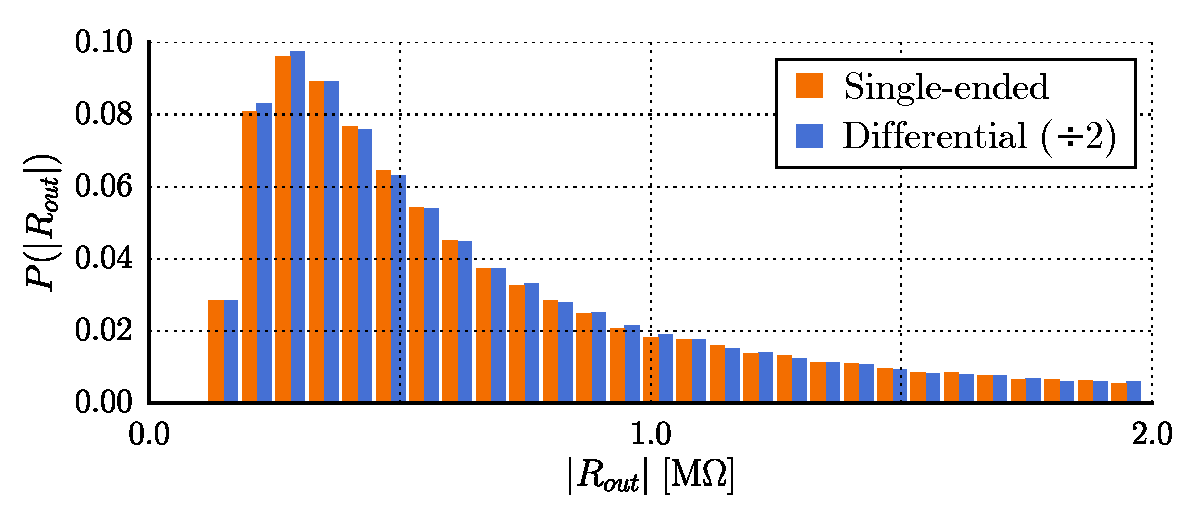
\includegraphics[scale=.55]{fig_mc_output_resistance.pdf}}}
\caption{\small Monte Carlo simulation of absolute DC output resistance for a resistor tolerance of 0.1\% and ideal op-amps. For each circuit, $10^5$ samples were generated. Note that the output resistance of the differential VCCS is twice as high as the single-ended VCCS but is scaled by a factor \vulgaronehalf~in this plot to allow easier visual comparison.}
\label{fig:mc_output_resistance}
\end{figure}

%%%%%%%%%%%%%%%%%%%%%%%%%%%%%%%%%%%%%%%%%%%%%%%%%%%%%%%%%%%%%%%%%%%%%%%%%%%%%%
\subsubsection{Proxy measurement of output impedance}
\label{sec:proxy_output_impedance}

When the output impedance of the VCCS reaches into the dozens of $\mega\ohm$, high precision instrumentation is required to obtain enough significant digits. In addition, the measurement is affected by the non-ideal behaviour of the op-amps, which causes $Z_{out}$ to be a finite, complex and frequency-dependent value.

Although either form of \briefeqlink{eq:z_out} thus requires the measurement of a complex load voltage (or current), in practice only the (scalar) magnitude is available with sufficient accuracy and precision. If we substitute magnitudes into \briefeqlink{eq:z_out}, we obtain an expression for a new, real-valued quantity $\hat{Z}_{out}$ (\briefeqlink{eq:z_out_quasi}), which is equal to the true magnitude $|Z_{out}|$ at DC, but begins to diverge for increasing frequency:
\begin{subequations}
\label{eq:z_out_quasi}
\begin{align}
\hat{Z}_{out} &= \frac{R_{L,a} R_{L,b} (|V_{L,b}| - |V_{L,a}|)} {|V_{L,a}|R_{L,b} - |V_{L,b}| R_{L,a}} \label{eq:z_out_quasi_volt} \\
&= \frac{|I_{L,b}| R_{L,b} - |I_{L,a}| R_{L,a}} {|I_{L,a}| - |I_{L,b}|} \label{eq:z_out_quasi_curr}
% & = \frac{I_{L,b} R_{L,b} - I_{L,a} R_{L,a}} {I_{L,a} - I_{L,b}} \label{eq:z_out_curr}
\end{align}
\end{subequations}
The quantity $\hat{Z}_{out}$ can be used to determine the full, complex output impedance $Z_{out}$, under the assumption that $Z_{out}$ can be modeled as a resistor $R_{out}$ in parallel with a capacitor $C_{out}$. In this case, $|V_L|$ can be written as:
\begin{align}
|V_L| = g_m V_{in,dif\!f}\frac{R_L\|R_{out}} {\sqrt{1 + (\omega (R_L\|R_{out}) C_{out})^2}} \label{eq:v_l_for_ref_circuit}
\end{align}

\begin{figure}[t!]

\begin{subfigure}{\textwidth}
\hspace{-4.8cm}\makebox[\textwidth][c]{%
\scalebox{.8}{%
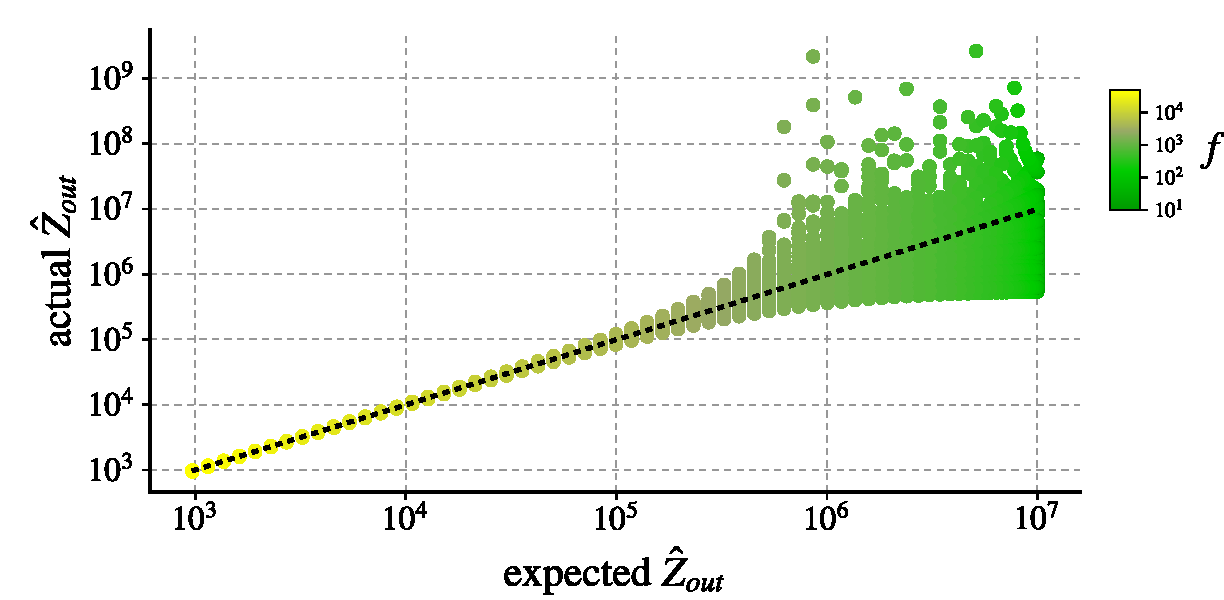
\includegraphics[scale=.55]{sensitivity_[method=voltage].pdf}}}
% \caption{\small abc}
\caption*{}
\label{fig:measurement_sensitivity_voltage}
\end{subfigure}

\begin{subfigure}{\textwidth}
\hspace{-4.8cm}\makebox[\textwidth][c]{%
\scalebox{.8}{%
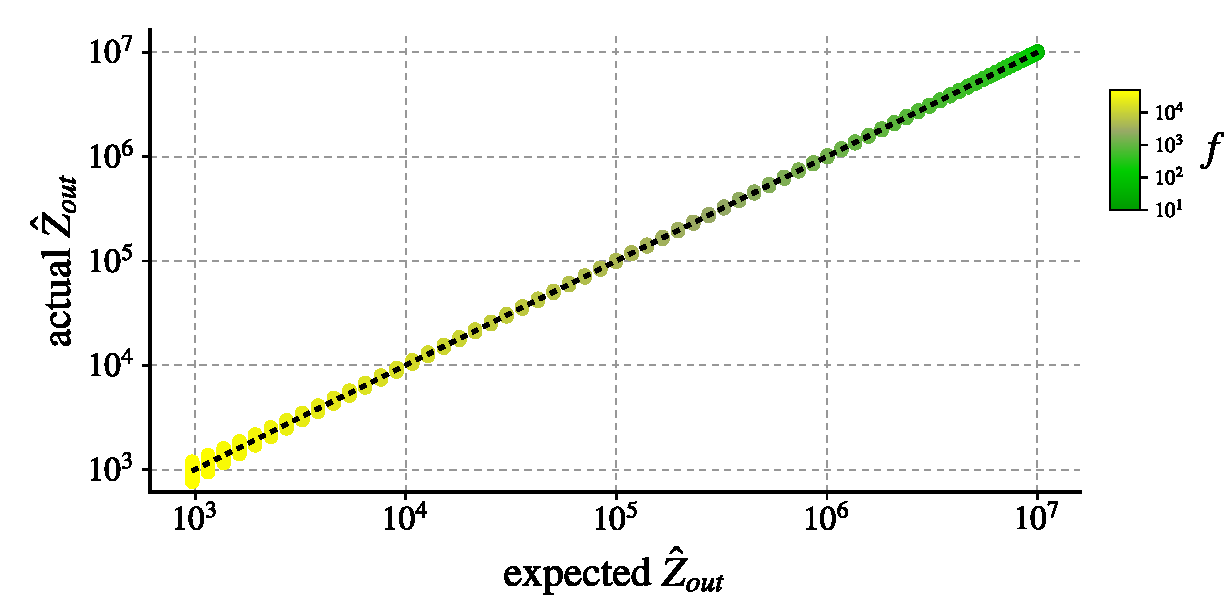
\includegraphics[scale=.55]{sensitivity_[method=current].pdf}}}
\caption*{}
% \caption{\small}
\label{fig:measurement_sensitivity_current}
\end{subfigure}

\caption{\small Sensitivity of the measured $\hat{Z}_{out}$ to tolerance of the probe resistors $R_{L,a}$ and $R_{L,b}$, for voltage-based method (top) and current-based method (bottom). For each point, colour indicates the frequency at which it was measured; impedance drops at higher frequencies due to the presence of $C_{out}$.}
\label{fig:measurement_sensitivity}
\end{figure}
This expression is substituted into \briefeqlink{eq:z_out_quasi_volt}, yielding a theoretical prediction for $\hat{Z}_{out}$ as a function of frequency, parameterised by $R_{out}$ and $C_{out}$. The resulting curves exhibit a typical RC lowpass filter shape, with plateau and roll-off (see solid lines in \brieffiglink{fig:output_resistance_empirical} for examples).

%%%%%%%%%%%%%%%%%%%%%%%%%%%%%%%%%%%%%%%%%%%%%%%%%%%%%%%%%%%%%%%%%%%%%%%%%%%%%%
\subsubsection{Effects of probe resistor tolerance}
\label{sec:probe_resistor_effects}

Measurement artefacts may be introduced as a consequence of tolerance in the component values of $R_{L,a}$ and $R_{L,b}$. For example, at DC, let $R_{L,a}=10~\kilo\ohm.$ If $R_{L,b}$ is assumed to be $11~\kilo\ohm$, but its actual in-circuit value is $15~\ohm$ larger, then a $1~\mega\ohm$ output resistance will be reported as $2.8~\mega\ohm$ by the voltage-based method (a relative error of 280\%), but as $0.985~\mega\ohm$ by the current-based method (a relative error of only 1.5\%).

To quantify the artefact magnitude across frequency $f$, we sample values for $R_{L,a}$ and $R_{L,b}$ from a uniform distribution, centered upon a mean of $10~\kilo\ohm$ resp. $11~\kilo\ohm$, and within a 0.1\% tolerance range. An output capacitance of $1~\nano\farad$ is assumed. We compute an ``expected'' $\hat{Z}_{out}$, on the basis of ideal load resistors, and an ``actual'' $\hat{Z}_{out}$, based on the samples. The actual value (vertical axis) is then plotted with respect to the expected value (horizontal axis). If the measurement were completely insensitive to tolerance in the resistors, the actual value would be precisely the same as the expected value, causing all points to fall exactly on the diagonal, indicated by the dashed black lines in \brieffiglink{fig:measurement_sensitivity}. Any vertical offset between a point and the diagonal corresponds to the measurement artefact introduced by tolerance in the probe resistors.

The voltage-based method (\brieffiglink{fig:measurement_sensitivity}, top panel) is most sensitive to variations in probe resistor values there where it matters most: in the region of highest output impedance. This makes it an unsuitable method for measuring the output impedance of a current source, which is generally characterised by high output impedance. The current-based method (\brieffiglink{fig:measurement_sensitivity}, bottom panel) also suffers from sensitivity to probe resistance, but this occurs at higher frequency and consequently at values of $\hat{Z}_{out}$ that are so low as to be outside the range of interest for a VCCS.

%%%%%%%%%%%%%%%%%%%%%%%%%%%%%%%%%%%%%%%%%%%%%%%%%%%%%%%%%%%%%%%%%%%%%%%%%%%%%%%
\section{Empirical results}
\label{sec:empirical-results}
%%%%%%%%%%%%%%%%%%%%%%%%%%%%%%%%%%%%%%%%%%%%%%%%%%%%%%%%%%%%%%%%%%%%%%%%%%%%%%%

\begin{figure}[b!]
\centering
\ctikzset{amplifiers/scale=1}
\scalebox{.75}{%
\begin{circuitikz}
	\node [op amp] (opamp) at (7.5, 1.49) {} ;
	\node [spdt, rotate=270, yscale=-1] (spdt) at (5.3, .4) {} ;

    \node [] (VLpos) at (4, -2.2) {};
% 	\node [label=right:$V_{L,pos}$] (VLneg) at (8, 2) {};
	\node [] (VLneg) at (8, 2) {};
	\node [] (VLnegmeas) at (12, 2) {};
	\node [] (op_vin_p) at (2, -2.2) {};
	\node [] (op_vin_n) at (2, 2) {};
	\node [] (op_vin_p2) at (1, -2.2) {};
	\node [] (op_vin_n2) at (1, 2) {};

	\node [] (vboxtr) at (-2., 1.4) {};
	\node [] (vboxbr) at (-2., -2.6) {};
	\node [] (vboxtl) at (1.5, 1.4) {};
	\node [] (vboxbl) at (1.5, -2.6) {};

	\draw[dashed] (vboxtr.center) to [short] (vboxbr.center) {};
	\draw[dashed] (vboxbr.center) to [short] (vboxbl.center) {};
	\draw[dashed] (vboxbl.center) to [short] (vboxtl.center) {};
	\draw[dashed] (vboxtl.center) to [short] (vboxtr.center) {};

	\draw (-.75, -2.2) to [american controlled current source, l=$g_m$] (-.75, 1) {}; % , i^>=$I$
	\draw (0.25, 1) to [generic, l=$Z_{out}$, *-*] (0.25, -2.2) {};
	\draw (2, 1) to [R, l=$R_{sens}$, i>^=$I_L$, -*] (5.3, 1) {};
	\draw (2, -2.2) to [short] (5.3, -2.2) {};
% 	\draw (2, -2.2) to [R, l=$R_{sens}'$, color=lightgray!50] (5.3, -2.2) {};
	\draw (spdt.out 1)+(0, .2) to [R, a=$R_{L,a}$, -*] +(0, -2) {};
	\draw (spdt.out 2)+(0, .2) to [R, l=$R_{L,b}$] +(0, -2) {};

	\draw (opamp.+) to +(-1, 0) {};
	\draw (opamp.-) -| +(-4.3, 0) to +(-4.3, 0) to [short, -*] (2, 1) {};

	% IA resistor
	\draw (opamp.-)+(0, -.1) to [R, resistors/scale=.5] +(0, -.85) {};
	\draw (opamp.-)+(0, -.1) to +(.35, -.1) {};
	\draw (opamp.-)+(0, -.85) to +(.35, -.85) {};

	% voltmeter
    \draw (opamp.out) -- +(0, 0) to +(0,-.25) to [rmeter, t=\large V] +(0, -1.25) node[rground] {};

 	\draw (5.621, -2.2) to [short] (5, -2.2) {};
	\draw (-.757, -2.2) to [short] (2, -2.2) {};
	\draw (-.757, 1) to [short] (2, 1) {};

% 	\draw (op_vin_n) to [short] (op_vin_n2) {};
% 	\draw (VLneg) to [short] (op_vin_n2) {};
% 	\draw (op_vin_p) to [short] (op_vin_p2) {};
\end{circuitikz}

}
\caption{\small Method for determining the output impedance of the VCCS. The dashed box indicates the non-ideal VCCS, which has a finite output impedance $Z_{out}$. As in \brieffiglink{fig:situation_sketch}, the ground node is assumed internal to $g_n$. An instrumentation amplifier measures the load current $I_L$ via the voltage drop across a sense resistor $R_{sens}$ while two load resistors, $R_{L,a}$ and $R_{L,b}$, are alternately connected.}
\label{fig:vccs_output_current}
\end{figure}

%%%%%%%%%%%%%%%%%%%%%%%%%%%%%%%%%%%%%%%%%%%%%%%%%%%%%%%%%%%%%%%%%%%%%%%%%%%%%%
\subsection{Description of the prototypes}
\label{sec:description_of_the_prototype}

Two prototype circuits were built to validate predictions from theory and simulation with empirical measurements. Circuits were constructed using surface-mount devices in SOIC-8 and 1206 ($3.2\times1.6~\milli\meter$) packages on a 1.6 mm dual layer FR-4 PCB with a ground plane on the bottom layer. Devices were battery-powered with a linearly regulated bipolar supply of $\pm15~\volt$.

%%%%%%%%%%%%%%%%%%%%%%%%%%%%%%%%%%%%%%%%%%%%%%%%%%%%%%%%%%%%%%%%%%%%%%%%%%%%%%
\subsubsection{Component selection}

All fixed resistors used in the circuit were rated at a tolerance of $0.1\%$ or better. The LT1211 (Analog Devices, USA) is used for op-amps.

%%%%%%%%%%%%%%%%%%%%%%%%%%%%%%%%%%%%%%%%%%%%%%%%%%%%%%%%%%%%%%%%%%%%%%%%%%%%%%
\subsubsection{Input drive signal}

The inputs of each VCCS were driven in antiphase, such that $V_{in,neg}=-V_{in,pos}$ at all times. For the single-ended supply, input voltages were buffered using additional op-amps configured as voltage followers.

%%%%%%%%%%%%%%%%%%%%%%%%%%%%%%%%%%%%%%%%%%%%%%%%%%%%%%%%%%%%%%%%%%%%%%%%%%%%%%
\subsubsection{Loop stability}

We used the ``lead'' compensation method for stability of the feedback loop, and found the optimal values by parameter sweeps in simulation, for each circuit individually, under a $Z_L=10~\kilo\ohm\|1~\micro\farad$ load condition, chosen to yield a DC output voltage close to the compliance voltage, and representing a worst-case capacitance, noting that higher capacitance is associated with decreased stability. In the single-ended VCCS, lead compensation is implemented by placing a feedback capacitor $C_{FB}=6.6~\pico\farad$ parallel to $R_2$ (see \brieffiglink{fig:single_ended_howland}); in the differential VCCS, two feedback capacitors $C_{FB,1}=C_{FB,2}=C_{FB}=3.3~\pico\farad$ are placed in parallel with $R_1$ and $R_3$, respectively (see \brieffiglink{fig:differential_howland}).

\begin{figure}[t!]
\begin{subfigure}{\textwidth}
\hspace{-4.6cm}\makebox[\textwidth][c]{%
\scalebox{.8}{%
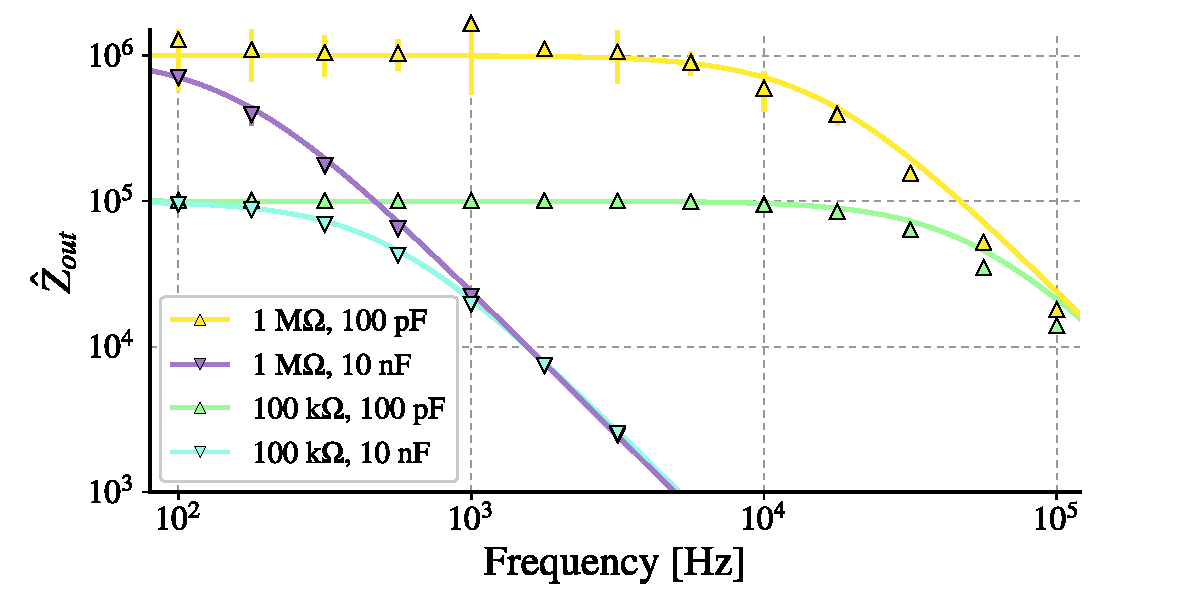
\includegraphics[scale=.6]{output_resistance_empirical_ref.pdf}}}
\caption*{}
\label{fig:output_resistance_empirical_ref}
\end{subfigure}
\ \\
\begin{subfigure}{\textwidth}
\hspace{-4.6cm}\makebox[\textwidth][c]{%
\scalebox{.8}{%
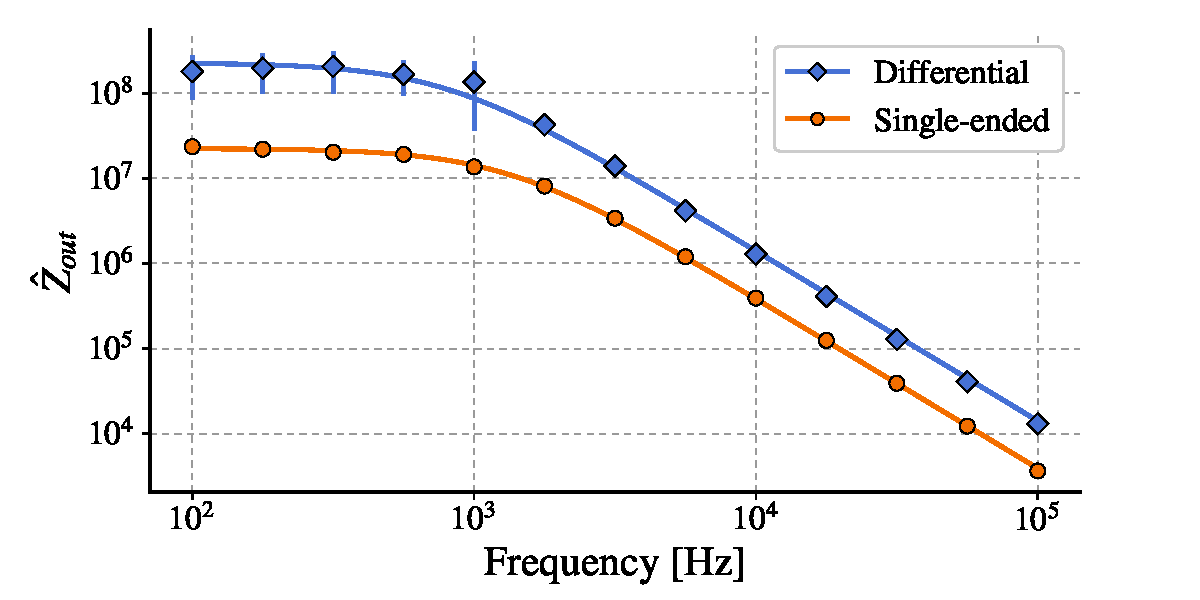
\includegraphics[scale=.6]{fig_output_resistance_empirical.pdf}}}
\caption*{}
\label{fig:output_resistance_empirical_meas}
\end{subfigure}
\caption{\small Empirical output resistance measurements for reference loads (top panel) and single-ended and differential VCCS circuits (bottom panel). Error bars due to measurement noise are plotted for each datapoint, but are visible only for the highest impedances.}
\label{fig:output_resistance_empirical}
\end{figure}


%%%%%%%%%%%%%%%%%%%%%%%%%%%%%%%%%%%%%%%%%%%%%%%%%%%%%%%%%%%%%%%%%%%%%%%%%%%%%%
\subsubsection{Measuring output current}

To measure actual delivered current, an instrumentation amplifier (INA128U, Texas Instruments, USA) was set up to measure voltage drop across a $10~\ohm$ resistor $R_{sens}$ placed in series with the load (\brieffiglink{fig:vccs_output_current}). The instrumentation amplifier was configured for a gain of 51, so a current of 1 mA yields a measured voltage of 0.51 V. For a 6-digit multimeter, this in turn yields a maximum theoretical measurable output impedance of $510~\mega\ohm$. Higher gain will improve the highest measurable impedance, but reduces the highest measurable frequency (here, 100 kHz) due to the finite gain-bandwidth product of the instrumentation amplifier.


%%%%%%%%%%%%%%%%%%%%%%%%%%%%%%%%%%%%%%%%%%%%%%%%%%%%%%%%%%%%%%%%%%%%%%%%%%%%%%
\subsubsection{Trimming}

To trim output resistance, $R_2$ in the single-ended, and $R_1$ and $R_3$ in the differential circuit were implemented as the series connection of a fixed resistor and a trimmer potentiometer. Trimming was performed as follows. The VCCS was set for a DC current of $1~\milli\ampere$. Two loads were alternately applied to the source: a short circuit, and a $10~\kilo\ohm$ resistor. The actual delivered current was measured, and the trimmer potentiometer was adjusted until these values converged. For the differential source, the trimming potentiometers were alternately adjusted in small increments until covergence.


%%%%%%%%%%%%%%%%%%%%%%%%%%%%%%%%%%%%%%%%%%%%%%%%%%%%%%%%%%%%%%%%%%%%%%%%%%%%%%
\subsection{Measurement of output impedance}
\label{sec:empirical_output_resistance}

To measure output impedance, the current-based method (\briefeqlink{eq:z_out_quasi_curr}) was used as described in \briefseclink{sec:output_impedance_measurement}. Resistor values $R_{L,a}=10~\kilo\ohm$ and $R_{L,b}=11~\kilo\ohm$ were selected to obtain an output voltage close to the compliance voltage, and for having a relatively small difference between them while taking finite measurement precision into account. A function generator and 6-digit digital voltmeter with frequency range up to $100~\kilo\hertz$ were set up for automated data acquisition via the IEEE~488 (``GPIB'') instrument bus. Samples which resulted in $\hat{Z}_{out}=\infty$ were discarded. This setup allowed us to reliably measure output resistance up to about $100~\mega\ohm$ (see variance bars in \brieffiglink{fig:output_resistance_empirical}).

The method was first validated using a reference circuit with known values. A function generator (sinusoidal voltage source) with $50~\ohm$ output impedance was connected in series with a resistor of known value: $100~\kilo\ohm$ or $1~\mega\ohm$. This is the Th\'{e}venin equivalent of a current source with an output resistance of the same value. Simultaneously, this ``current source'' was loaded with a load capacitance $C_L=100~\pico\farad$ or $10~\nano\farad$, simulating the output capacitance $C_{out}$. This ``current source'' was then characterised using the same method. Results are shown in the top panel of \brieffiglink{fig:output_resistance_empirical}. In this figure, empirical data is represented as points, while predicted values, based on the known $R_{out}$ and $C_{out}$, are plotted as solid lines. The limit of voltmeter resolution is especially visible in the $1~\mega\ohm$ condition, due to the large Ohmic voltage drop resulting in a very small load current. Overall, a good match between the empirical data and theoretical predictions can be observed, validating the accuracy and precision of our methodology.

\begin{table}[t!]
\centering
\bgroup
\def\arraystretch{1.3}%  1 is the default, change whatever you need
\newcolumntype{a}{>{\hsize=4\hsize}X}
\newcolumntype{b}{>{\hsize=13\hsize}X}
\newcolumntype{c}{>{\hsize=5.5\hsize}X}
\begin{tabularx}{5.7cm}{ a|c|c }
 & Single-ended & Differential\\
\hline
$R_{out}$ & $22.5~\mega\ohm$ & $249~\mega\ohm$ \\
$C_{out}$ & $245~\pico\farad$ & $131~\pico\farad$ \\
\end{tabularx}\egroup
\caption{\small Fitted values for resistive and capacitive components of the output impedance.}
\label{tbl:Z_hat_out_curve_fit}
\end{table}

Next, the VCCS prototypes were characterised. The bottom panel of \brieffiglink{fig:output_resistance_empirical} shows both the empirical measurements (as points), and the theoretical prediction based on curve fitting (as solid lines). To perform curve fitting, the Nelder-Mead algorithm \cite{neldermead} was used to find the $R_{out}$ and $C_{out}$ that minimise an error measure, defined as the squared difference between the (base 10) logarithm of the predicted, and logarithm of the empirical $\hat{Z}_{out}(f)$, summed over all measured frequencies $f$. Fitting was done independently for each circuit. Overall, good agreement between empirical data and the fitted curves is observed in \brieffiglink{fig:output_resistance_empirical}, supporting the resistive-capacitive model of VCCS output impedance. Results of the fit are repeated in \brieftbllink{tbl:Z_hat_out_curve_fit} to allow a more precise quantitative comparison. The DC output resistance of the differential source is seen to outperform the single-ended source by a factor of more than 2, exceeding the improvement that was predicted based on theory in \briefseclink{sec:monte_carlo}. Because we trim each circuit towards the singularity point where $R_{out}$ approaches infinity, sensitivity to trim near this point is extremely high, explaining the variance. In contrast, the capacitive part of the output impedance $C_{out}$ comes much closer to a factor 2 improvement from the single-ended to the differential circuit. This can be attributed to the high-frequency behaviour being dominated by the $C_{FB}$ capacitors, which were chosen a factor of 2 different in value.


%%%%%%%%%%%%%%%%%%%%%%%%%%%%%%%%%%%%%%%%%%%%%%%%%%%%%%%%%%%%%%%%%%%%%%%%%%%%%%
\section{Conclusion}
\label{sec:conclusion}
%%%%%%%%%%%%%%%%%%%%%%%%%%%%%%%%%%%%%%%%%%%%%%%%%%%%%%%%%%%%%%%%%%%%%%%%%%%%%%

On the basis of analysis and simulation, we conclude that only the current-based method for measuring VCCS output impedance has practical application value (\briefseclink{sec:probe_resistor_effects}). In addition, we find empirically that we can infer the full, complex-valued $Z_{out}$ on the basis of the proxy measurement of $\hat{Z}_{out}$ (\briefseclink{sec:proxy_output_impedance}). Our method is suitable for VCCS circuits with a fully differential output, and was able to provide reliable data up to about $100~\mega\ohm$ at frequencies up to $100~\kilo\hertz$.

In general, for electronics that is used \emph{in vivo} in medicine or research, an abundance of caution should be exercised. A higher voltage range should be used with care; depending on operating conditions, keeping the voltage low can contribute to safety \cite{pmid15661300}. Output impedance measurement of the VCCS should be complemented by time-domain transient validation, temperature stability testing, common-mode output voltage measurements, and so on. Additional safety margins (such as on loop stability), low-current fuses and other passive and active protection mechanisms are crucial steps in going from the core VCCS circuit to a ready-to-use, clinical or research tES device, and indicate potential directions for future research.
\balance

\bibliographystyle{IEEEtran}
\bibliography{conference_101719}

\end{document}

